\subsubsection{Conservation Laws}

\paragraph{The Method of Characteristics}

\subparagraph{Integral Surface}

Consider the general quasilinear first order PDE:
\begin{equation}
a(x,y,u)u_x + b(x,y,u)u_y = c(x,y,u)
\end{equation}
We note that the vector field $( -u_x, -u_y, 1)^T$ would be orthogonal to the solution $u(x,y)$ everywhere. Therefore the vector field $(a, b, c)^T$ is perpendicular to $( -u_x, -u_y, 1)^T$ thus must lie in the tangent plane of $u(x,y)$. Surfaces that are tangent to a vector space is called \textit{integral surfaces}, hence to find the solution we want to find the integral surfaces of $u(x,y)$.

We do this by:

\begin{framed}
\textbf{Method of Characterisitcs}\\
\begin{enumerate}
\item Parametrize the inital condition $\Gamma(r)$
\item Find integral curves $\chi$ starting from one instance of the initial condition(at some $r$) by solving a system of ODE.
Concretely, suppose $\chi(s) = (x(s),y(s),z(s))$ is a parametrization of the integral curves, then it must satisfy that:
\begin{equation}
\begin{cases}
\frac{dx}{ds}&=a(x,y,u) \\
\frac{dy}{ds}&=b(x,y,u) \\
\frac{dz}{ds}&=c(x,y,z) \\
\end{cases}
\end{equation}
on some small $|t -t_0|<\delta$.  The resulting integral curves are functions of $r,s$ where $r$ specifies where the evolution start and $s$ specifies how much the integral curve grow away from the $\Gamma$.


\item Compute the integral surface as a continuous union by replacing $r,s$ with $x,y$
\end{enumerate}
\end{framed}

\begin{example}[Constant Wave-speed Advection]Consider the equation $u_t+cu_x=0$ with the initial condition $u(t,0)=\exp( -x^2)$. We parametrize the initial condition as $(t,x,z)=(0,r,\exp( -r^2))$. Fix $r$, the system is:
\begin{equation}
\begin{cases}
   \frac{dt}{ds}&=1 \\
   \frac{dx}{ds}&=c \\
   \frac{dz}{ds}&=0 \\
   \end{cases}
   \Longrightarrow
   \begin{cases}
   t(r,s)=s+C(r) \\
   x(r,s)=cs+D(r)\\
   z(r,s)=E(r) \\
   \end{cases}
\end{equation}
Substituting the initial condition, we get:
\begin{equation}
\begin{cases}
   t(r,s)=s \\
   x(r,s)=cs+r\\
   z(r,s)=\exp(-r^2) \\
   \end{cases}
\end{equation}
But now $r=x -cs=x -ct$ hence we get the solution:
\begin{equation}
u(t,x)=\exp(-(x-ct)^2)
\end{equation}
Visualizing the solution:

\begin{figure}[!htbp]
\centering
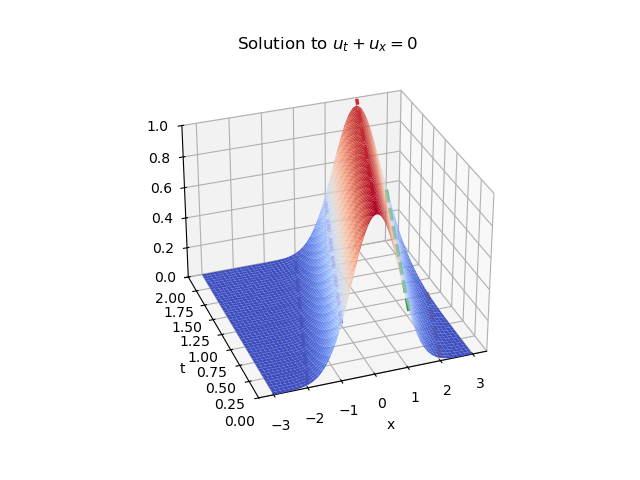
\includegraphics[width=0.7\linewidth]{files/ex1-12fb0a22df1e48f3994c66c3b0db0eda.png}
\caption*{We showed the special case when $c=1$, the lines are the integral curves above. In this special case the value of $z=u(x,y)$ is fixed on the curve.}
\end{figure}

\end{example}\paragraph{The Finite Volume Method}

\subparagraph{Hyperbolic Conservation Law}

For simplicity, we consider the homogenous case:
\begin{equation}
u_t + a(t,x)u_x = 0
\end{equation}
If we discretize the spatial domain into an array of contiguous cells called \textit{control volumes},
we can see that the equation encapsulate a sense of \textit{conservation}. Suppose $[a,b]$ is a cell of interest, integrate the equation by parts results in :
\begin{equation}
\frac{d}{dt}\int_{a}^b u  dx = \underbrace{a(t,a)u(t,a)}_{\text{flux in}}-\underbrace{a(t,b)u(t,b)}_{\text{flux out}} - \underbrace{\int_a^b a_x(t,x)udx}_{\text{source/disspation}}
\end{equation}
In particular, if we have $a(t,x)=a(t)$, then we have no source and disspation. This motivates us to define:

\begin{definition}[Hyperbolic Conservation Law]There are two subclasses, \textbf{strict conservation law}(with no source term) and \textbf{balance law}(conservation law with source term).

\begin{enumerate}
\item Conservation Law

\begin{equation}
u_t + (f(u))_x = 0
\end{equation}


\item Balance Law

\begin{equation}
u_t + (f(u))_x = g(u,x,t)
\end{equation}
\end{enumerate}

\end{definition}For a simple strict conservation law we have:
\begin{equation}
\frac{d}{dt}\int_a^b u = \underbrace{f(u(a,t))}_{\text{flux in}}-\underbrace{f(u(b,t))}_{\text{flux out}}
\end{equation}
It is clear that:

\begin{proposition}The general homogenous transport equation $u_t+a(x,t)u_x=0$ is a strict conservation law iff $a(x,t)=a(t)$

\end{proposition}\subparagraph{The idea behind finite volume}

\begin{framed}
\textbf{Discretization}\\
Finite volume discretize the space into cells $x_i, i\in \mathbb{N}$ being the cell center and $x_{i -1/2},x_{i+1/2}$ being the faces of the cell.
\end{framed}

Finite volume method utillise the conservation structure of the equation. Specifically, we enforce that conservation law holds at each cell $[x_{i -1/2},x_{i+1/2}]$\newline
\begin{equation}
\int_{t_j}^{t_{j+1}}\left\{ \int_{x_{i-1/2}}^{x_{i+1/2}} \left[ u_t + (f(u))_x -g\right]dx \right\}dt=0
\end{equation}